\section{Задание}

\subsection{Работа с поляризатором и закон Малюса}
Для определения поляризации, предлагаю импользуяпосмотрев на 
черное стекло через полризатор можно найти минимум $\mathfrak{I}$. 
В этом положении поляризатор перпенперпендикурярен полскости отражения.

Такким образом направления первого поляризатора у меня получилось 
$20^\circ$. Используя поляризатор можем найти поляризацию источника. 

Теперь я беру 2 поляризатор и снова нахожу минимум 
относительно 1 поляризатора. Вращая на угол $\varphi$ от 
найденного $min$ проверяем закон. 

\begin{figure}[h]
    \centering
    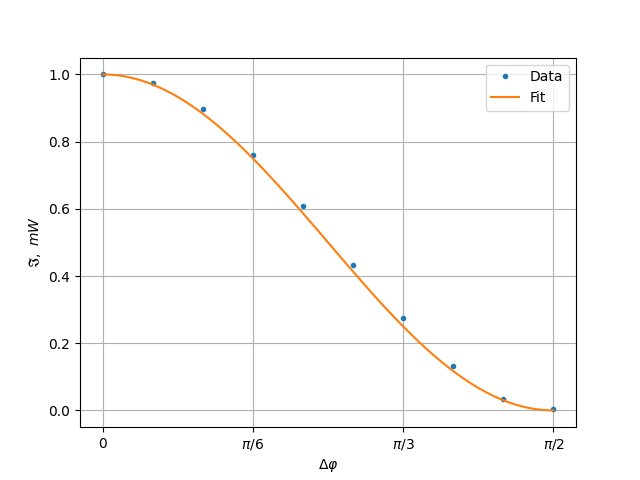
\includegraphics[trim={0 0 0 0},clip,width=\textwidth]{Ex_1/Task_1_1.png}
     \caption{Результаты измерений, данные отнормированны на $\mathfrak{I}_{max}$}
    \label{Task_1_1}
\end{figure}

\subsection{Работа с пластинками $\cfrac{\lambda}{4}, \ \cfrac{\lambda}{2}$}

Для определения направления пластинок 
$\cfrac{\lambda}{2}, \ \cfrac{\lambda}{4}$, предлагаю потавтить 
два поляризатора в пложение $\Delta \varphi = \cfrac{\pi}{2}$. 
Поле вмежду ними ставим неизветные нам пластинки в ращаем до 
$\mathfrak{I}_{min}$. Это означает, что оси пластинок совпали 
с направлением первого поляризатора. Для того чтобы отличить 
$\cfrac{\lambda}{2}, \ \cfrac{\lambda}{4}$ провернем на 
$\cfrac{\pi}{4}$ относительно наденного нами минимума. 
Теперь вращаем второй поляризатор, ели у нас пластика $\cfrac{\lambda}{2}$ 
то будет существовать ярко выраженный $min \land max$ или другими словами 
$\vartheta = 1$ ели же попалась пластинка $\cfrac{\lambda}{4}$ то $\vartheta = \cfrac{1}{2}$   

но наши пластинки не идеальны поэтому давайте найдем рельную видность.
Для пластинки $\cfrac{\lambda}{4}$ получил 
$\mathfrak{I}_{max} = 1.1 W, \ \mathfrak{I}_{min} = 0.702 W \implies \vartheta = 0.23$
Оналогично для $\cfrac{\lambda}{2}: \ \mathfrak{I}_{max} = 1.1 W, \ 
\mathfrak{I}_{min} = 0.702 W \implies \vartheta = 0.99 \to 1$.











